\documentclass{article}

\usepackage{ijcai15}
\usepackage{times}
\usepackage{url}
\usepackage{graphicx}
\usepackage{multirow}

\newenvironment{packed_enum}{
\begin{enumerate}
  \setlength{\itemsep}{1pt}
  \setlength{\parskip}{0pt}
  \setlength{\parsep}{0pt}
}{\end{enumerate}}

\title{Zoom: a corpus of natural language descriptions of map locations}
%\thanks{Thanks.}}
\author{no name \\
no institution\\
no location \\
no email}

\begin{document}

\raggedbottom

\maketitle

\begin{abstract}
This paper describes 
an experiment  to elicit referring expressions
from human subjects 
for research in natural language generation and related fields,
and preliminary results of a computational model 
for the generation of these expressions.
Unlike existing resources of this kind, 
the resulting data set - the Zoom corpus of natural language descriptions of map locations -
takes into account a domain that is significantly closer to real-world applications, 
and addresses more complex situations of reference, including
contexts with different levels of detail, and
instances of singular and plural reference 
produced by a relatively large number of speakers 
in both Spanish and Portuguese languages.
\end{abstract}


%%%%%%%%%%%%%%%%%%%%%%%%%%%%%%%%%%%%%%%%%%%%%%%%%%%%%%%%%%%%%%%%%%%%%%%%%%%%%%%%%%%%%%%%%%%%%%%%%%%%%%%%%%%%%%%%%%%%%%%%%%%%%%%%%%%%%%%%%%%%%%%%%%%%%%%%%%	       >2
\section{Introduction}
%%%%%%%%%%%%%%%%%%%%%%%%%%%%%%%%%%%%%%%%%%%%%%%%%%%%%%%%%%%%%%%%%%%%%%%%%%%%%%%%%%%%%%%%%%%%%%%%%%%%%%%%%%%%%%%%%%%%%%%%%%%%%%%%%%%%%%%%%%%%%%%%%%%%%%%%%%	       >2

In Natural Language Generation (NLG), Referring Expression Generation (REG) is the computational task of producing adequate natural language descriptions (e.g., pronouns, definite descriptions, proper names etc.) of domain entities. In particular, the issue of how to determine the semantic content of definite descriptions (e.g., `the Indian restaurant on 5th street', `the restaurant we went to last night', `the large white building across the car park' etc.) has received significant attention in the field, and it is the focus of the present paper.

{\it ROMI-(more motivation...) Every system that have a natural language generator(NLG) needs a referring expression generator(REG), the quality of this REG system can do significant difference between a bot system and a system that produce language as people do. For example a system of taxi-car needs a GPS for navigation, that GPS could use a GRE system which can be more natural using a software to generate the RE.}

{\it ROMI- Now we are focusing in the REG algorithm.} The input to a REG algorithm is a context set $C$ containing an intended referent $r$ and a number of distractor objects. All objects are represented as attribute-value pairs, as in ({\em type-restaurant}) or ({\em on-5thstreet}). The expected output is a {\em uniquely identifying} list $L$ of properties known to be true of $r$ so that $L$ distinguishes $r$ from all distractors in $C$ \cite{incremental}. Properties are selected for inclusion in $L$ according to multiple - and often conflicting - criteria, including discriminatory power (i.e., the ability to rule out distractors), domain preferences and many others. For a review of the research challenges in REG, we report to \cite{survey}.


{\it ROMI-- they tell that the concept of minimal RE was not in the paper- also of sobrespecifications, I thing those concepts can be here.
A RE can contain a lot of properties, even considering a particular interlocutor you can give many RE for the same targer. A mininal RE is an expression that includes the minimal caracteristics to indentify the target in the scene into account and for a particular interlocutor. In constrast to that, a RE is overspecified when it includes more properties than the minimal necesary to identify the target. }

Existing approaches to REG largely consist of algorithmic solutions, many of which have been influenced by, or adapted from, the Dale \& Reiter Incremental algorithm in \cite{incremental}. The use of machine learning (ML) techniques, by contrast, seems to be less frequent than in other NLG tasks and in related fields, although a number of exceptions do exist (e.g., \cite{jordan,speaker-dependent,viethen-phd,thiago-svm}). 

A possible explanation for the small interest in ML for REG may be the relatively low availability of suitable data. While research in many fields may benefit from the wide availability of text corpora (e.g., obtainable from the web), research in REG usually requires highly specialised data  - hereby called REG corpora - conveying not only referring expressions produced by human speakers, but also a fully-annotated representation of the context (i.e., all objects and their semantic properties) within which the expressions have been produced. Examples of REG corpora include TUNA \cite{tuna-corpus}, GRE3D3 \cite{gre3d3}, and Stars \cite{stars-mutual-disamb}. 

REG corpora are useful both to gain general insights on human  language production, and to benefit from data-intensive computational techniques such as ML. However, being usually the  final product of controlled  experiments involving human subjects, resources of this kind tend to address highly specific research questions. For instance, GRE3D3 is largely devoted to the investigation of relational referring expressions in simple visual scenes involving geometric shapes, as in `the large ball next to the red cube'. As a result, and despite the usefulness of these resources to a large body of work in REG, further research questions will usually require the collection of new data.

In this paper we present a new resource of this kind - the Zoom corpus of referring expressions - that has been collected for research purposes, and which is intended to open a number of new opportunities of research in REG. First of all, the Zoom corpus focuses on situations of reference in a domain that is considerably closer to real-world applications (namely, map images of existing cities). The target descriptions of map locations involve both singular and plural reference, and make extensive use of relational properties (e.g., `the restaurant on 5th street'). Moreover, map scenes are represented with different degrees of detail represented by zoom levels, which will allow the future investigation of the issue of REG from different input knowledge bases. 

Second, unlike existing REG corpora, the Zoom corpus contains descriptions produced both in Spanish and Portuguese. This will allow (to the best of our knowledge, for the first time) a comprehensive study of the REG surface realisation subtask in these languages. Moreover, the corpus has been elicited from a considerably large number of subjects, which will enable research on the issues of between-speakers and within-speakers variation that have recently played a prominent role in the research in REG \cite{trainable-speaker,romina-coling,non-det}.

In addition to the experiment that produced the Zoom corpus and its structure, the paper will also describe the results of a machine learning approach to REG using the corpus. This is intended to provide a first baseline for future research using Zoom data.

%The rest of this paper is structured as follows. Section \ref{sec-background} describes related work on REG corpora. Section \ref{sec-experiment} describes the experiment design, and the data collection and annotation procedures. Section \ref{sec-eval} presents preliminary evaluation work using a SVM-based approach to REG, and Section \ref{sec-final} presents our final remarks.



%%%%%%%%%%%%%%%%%%%%%%%%%%%%%%%%%%%%%%%%%%%%%%%%%%%%%%%%%%%%%%%%%%%%%%%%%%%%%%%%%%%%%%%%%%%%%%%%%%%%%%%%%%%%%%%%%%%%%%%%%%%%%%%%%%%%%%%%%%%%%%%%%%%%%%%%%%	       
\section{Background}
%%%%%%%%%%%%%%%%%%%%%%%%%%%%%%%%%%%%%%%%%%%%%%%%%%%%%%%%%%%%%%%%%%%%%%%%%%%%%%%%%%%%%%%%%%%%%%%%%%%%%%%%%%%%%%%%%%%%%%%%%%%%%%%%%%%%%%%%%%%%%%%%%%%%%%%%%%	       
\label{sec-background}

In this section we briefly discuss a number of REG corpora publicly available for research purposes, and how these resources compare to our current work.

TUNA \cite{tuna-corpus} was the first prominent REG corpus to be made publicly available for research purposes. The corpus was developed in a series of general-purpose controlled experiments, containing 2280 descriptions produced by 60 speakers in two domains (1200 descriptions of furniture items and 1080 descriptions of people's photographs). TUNA does not contain relational descriptions, and it is possibly the only resource of this kind to include situations of reference to sets. The TUNA corpus has been extensively used in a series of shared tasks \cite{reg2009}.

GRE3D3 and its extension GRE3D7 \cite{gre3d3,gre3d7} were developed in a series of web-based experiments primarily focussed on the study of relational descriptions. GRE3D3 contains 630 descriptions produced by 63 speakers, and GRE3D7 contains 4480 descriptions produced by 287 speakers, making it the largest of its kind to date. The GRE3D domain consists of simple visual scenes containing only two kinds of objects (boxes and spheres) with limited variation in colour and size. In each scene, there is only one possible spatial relation between target and the nearest landmark. Both corpora contain atomic and relational descriptions.

Stars \cite{stars-mutual-disamb} and its extension Stars2 were collected for the study of referential overspecification (particularly in the case of relational descriptions). Stars was developed in a pilot web-based experiment, containing 704 descriptions produced by 64 speakers.  The more comprehensive Stars2 data set was produced in dialogue situations involving subject pairs, and it contains 884 descriptions produced by 56 speakers. Both domains make use of simple visual scenes containing up to four object types (e.g., stars, boxes, cones and spheres) with limited variation in colour and size. Differently from other REG corpora, however, Stars/2 includes a considerable number of complex situations of reference involving up to three objects, as in `the box near the sphere, next to the cone'. 

{\it ROMI-- they said that our system fault in compare with other systems.. here that comparison should be add}
Despite their usefulness and general contribution to the research in REG, the above domains are still at a certain distance from the kinds of visual scene that might be required for a practical, real-world application, {\it ROMI that distance is that we try to minimize, our corpus is from maps-locations, it is a domain that is usual to speak about for people, it can be use in navigations systems, recomending systems, etc.} {\it ROMI --without this phrase The need for additional complexity and/or realism, and}{\it ROMI-add The possibility of aboid the task of surface realisation between languages, is another point in favor of the Zoom corpus} {\it ROMI-- with out this phrase our own interest in the surface realisation task for the Spanish and Portuguese languages, has led us to build a new computational resource of this kind: the Zoom corpus of natural language descriptions of map locations.}{\it Another difference that do the Zoom corpus unique is that we have images in 2 degree of zoom, it is for the same target object we obtain how people reference to it in both levels of zoom. Our corpus also have considered plural and singular targets as TUNA does}.

 This work is described in the next sections. Further discussion on the differences between the Zoom corpus and existing resources is presented in Sec. \ref{sec-annotation}. 


%%%%%%%%%%%%%%%%%%%%%%%%%%%%%%%%%%%%%%%%%%%%%%%%%%%%%%%%%%%%%%%%%%%%%%%%%%%%%%%%%%%%%%%%%%%%%%%%%%%%%%%%%%%%%%%%%%%%%%%%%%%%%%%%%%%%%%%%%%%%%%%%%%%%%%%%%%	       
\section{Experiment}
%%%%%%%%%%%%%%%%%%%%%%%%%%%%%%%%%%%%%%%%%%%%%%%%%%%%%%%%%%%%%%%%%%%%%%%%%%%%%%%%%%%%%%%%%%%%%%%%%%%%%%%%%%%%%%%%%%%%%%%%%%%%%%%%%%%%%%%%%%%%%%%%%%%%%%%%%%	       
\label{sec-experiment}

In this section we describe the corpus characteristics, the participants, and the procedure of data collection and annotation. We also discuss here the issues associated to collecting natural language descriptions in a domain that is significantly closer to real-world applications in a web-based experiment.   

\subsection{Overview}

We designed a web-based experiment to collect natural language descriptions of map locations in both Spanish and Portuguese. The collected data set constitutes a corpus of referring expressions for research in REG and related fields. 

The situations of reference under consideration make use of map scenes in two degrees of detail (represented by low and high zoom levels), addressing both singular and plural descriptions, and taking into account a large number of subjects (about 100 speakers in each language). A fragment of the experiment interface is shown in {\it ROMI- if there is space, I will like to put here 2 more images of plural examples}Fig.~\ref{fig-interface} whit an image with low level of zoom, and~\ref{fig-with-zoom1} with high level of zoom for the same target.

\begin{figure}[ht]
\begin{center}
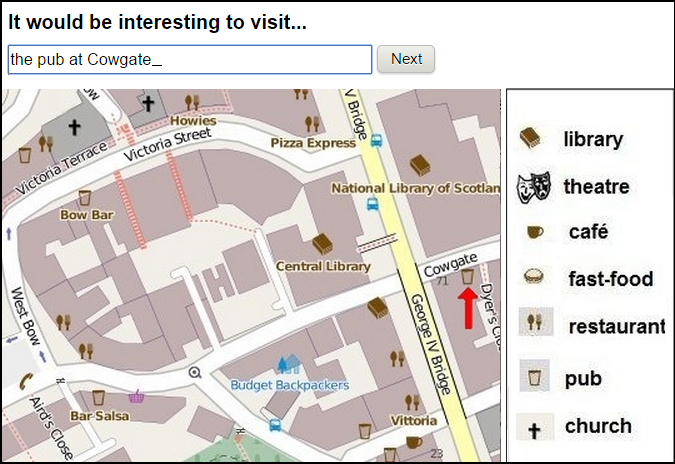
\includegraphics[width=8.5cm]{figures/interface.png}\\[0pt]
\caption{Experiment interface}
\label{fig-interface}
\end{center}
\end{figure}

\begin{figure}[ht]
\begin{center}
\fbox{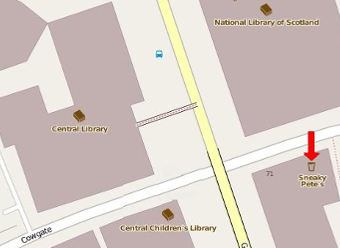
\includegraphics[width=8.3cm]{figures/with-zoom.jpg}}\\[0pt]
\caption{Map with a more detailed zoom level}
\label{fig-with-zoom1}
\end{center}
\end{figure}

%.....................................
\subsection{Subjects}
%.....................................

Volunteers were recruited upon  invitation sent by email and social networks. The Portuguese portion of the corpus had 93 participants, being 66 (71.0\%) male and 27 (29.0\%) female. The Spanish corpus had 85 participants, being 59 male (69.4\%) and 26 female (30.6\%).


%.....................................
\subsection{Procedure}
%.....................................

Subjects received a web link to the on-line experiment interface (similar to Fig. \ref{fig-interface}) with self-contained instructions. Subjects were required to select the language of the experiment (Portuguese, Spanish) and were briefed on the purpose of the experiment. Age and gender details were collected for statistical purposes. The experiment consisted of a series of map images presented in random order, one by one.{\it ROMI-clean english A progress bar was showing the progress level of the experiment.} 

Each map scene showed a particular location (e.g., a restaurant, pub, theatre etc.) pointed by an arrow  {\it ROMI-(or two locations pointed by arrows in plural target)}. For each scene, subjects were required to imagine that they were giving travel advice to a friend and to complete the sentence `It would be interesting to visit...' with a description of the location pointed by the arrow {\it ROMI-(or the arrows in plural target)}. After pressing a `Next' button, another stimuli was selected at random until the end of the experiment. 

The first two images were fillers solely intended to make subjects familiar with the experiment setting, and the corresponding responses were not recorded. Incomplete trials, and ill-formed descriptions, were also discarded. {\it ROMI-add } The concept of incomplete trials and ill-formed description will be explain in  Section~\ref{sec-problems} 



%.....................................
\subsection{Materials}
%.....................................

The experiment made use of the purpose-built interface illustrated in Fig. \ref{fig-interface} and a set of map images obtained from OpenStreetMap\footnote{\url{openstreetmap.org}}. These consisted of fragments of maps of the city centre of Madrid (for the Spanish portion of the corpus) and Lisbon (for the Portuguese portion). 

For each city, 10 map locations were used. Each location was shown with a low and a high zoom levels, making 20 images in total. In both low and high zoom levels  the intended target was kept the same, but the more detailed version would of course display a larger number of distractors and additional details in general. In addition to that, certain street and landmark names might not be depicted at different zoom levels.

Half images showed a single arrow pointing to one map location (i.e., requiring a single description as `the restaurant on Baker street'), whereas the other half showed two arrows pointed to two different locations (and hence requiring a reference to a set, as in `the restaurants near the museum'
{\it ROMI- or `the restaurant near the museum and the restaurant near to the Church') }. 


%.....................................
\subsection{Data Collection and Annotation}
%.....................................
\label{sec-annotation}

The experiment website was kept online until 100 complete trials were obtained for Portuguese and 80 complete trials were collected for Spanish. Upon manual verification, 602 ill-formed Portuguese descriptions and 366 Spanish descriptions were discarded. Thus, the Portuguese portion of the corpus consists of 1358 descriptions while the Spanish portion contains 1234 referring expressions. In Section~\ref{sec-problems} we describe the criteria by which descriptions were considered ill-formed. We also discuss the challenges faced when collecting natural language descriptions in a web-based experiment for a domain that is significantly closer to real-world applications than existing REG corpora. 

In the Portuguese portion of the data, 78.6\% of the descriptions include relational properties. In addition to that, 36.4\% were minimally distinguishing, 44.3\% were overspecified, and  19.3\% were underspecified. In the Spanish portion of the data, 70\% of the descriptions include relational properties. Moreover, 35\% were minimally distinguishing, 40\% were overspecified, and 25\% were underspecified. Underspecified descriptions as well as relational descriptions are not common in existing REG corpora - certainly not in this proportion.  
% I (Luciana) commented this part out because I don't understand it. 
%and will most likely represent an upper bound for REG algorithms intended to generate descriptions in this domain. 

Table \ref{tab-comparison} presents a comparison between the collected data and existing REG corpora. The domain information represents the number of possible atomic attributes and relations in each corpus. The information on TUNA and Zoom descriptions is based on the singular portion of each corpus only. This represents the average description size (in number of annotated properties) and properties usage, which is taken to be  the proportion of properties that appear in the description over the total number of possible properties. From a REG perspective, larger description sizes and lower usage scores are likely to represent more complex situations of reference.

\begin{table}[ht]
\begin{center}
\footnotesize{
\caption{Comparison with existing REG corpora}
\label{tab-comparison}
\begin{tabular} {  l c c c c}
\hline
\multicolumn{1}{c}{}
&\multicolumn{2}{c}{Domain}
&\multicolumn{2}{c}{Descriptions}\\
Corpus											& Attributes			& Relations			& Avg.size	& Usage \\
\hline
TUNA-Furniture							& 4								& 0							&	3.1				& 0.8   \\
TUNA-People									& 10							& 0							& 3.1				& 0.3   \\
GRE3D3											&	9								& 1							& 3.4				& 0.3   \\
GRE3D7											&	6								& 1							& 3.0				& 0.4   \\
Stars												&	8								& 2							& 4.4				& 0.4   \\
Stars2											& 9								& 2							& 3.3				& 0.3   \\
Zoom-Pt											& 19							& 7							& 6.7				& 0.3   \\
Zoom-Sp											& 19							& 7							& 7.2				& 0.3   \\
\hline
\end{tabular}
}
\end{center}
\end{table}


Annotation was performed as follows. Each referring expression was modeled as conveying a description of the main target object and, optionally, up to four descriptions of related landmarks. The annotation scheme consisted of three target attributes, four landmark attributes for each of the four possible landmark objects, and seven relational properties (no RE was found in the corpus with more than four landmark objects). This makes 26 possible attributes for each referring expression. In the case of plural descriptions (i.e., those involving two target objects), this attribute set is doubled.

Every object was annotated with the atomic attributes {\em type}, {\em name} and {\em others} and, in the case of landmark objects, also with their {\em id}. In addition to that, seven relational properties were considered: {\em in/on/at}\footnote{The three prepositions were aggregated as a single attribute because they have approximately the same meaning in the languages under consideration}, {\em next-to}, {\em right-of}, {\em left-of}, {\em in-front-of}, {\em behind-of}, and the multivalue relation {\em between} intended to represent `corner' relations. 

Possible values for the {\em type} and {\em name} attributes are predefined by each referential context. The {\em others} attribute may be assigned any string value, and it is intended to represent any non-standard piece of information conveyed by the referring expression. For the spatial relations, possible values are the object identifiers available from each scene.

The collected descriptions were fully annotated by two independent annotators. After completion, a third annotator assumed the role of judge and provided the final annotation. Since the annotation scheme was fairly straightforward (i.e., largely because all non-standard responses were simply assigned to the {\em others} attribute), agreement between judges as measured by Kappa \cite{kappa} was 84\% at the attribute level. 

Both referential contexts and referring expressions were represented in XML format using a simplified version of the XML format adopted in the TUNA corpus \cite{tuna-corpus}. Descriptions were grouped into TRIAL nodes containing general information about each subject (i.e., id, age and gender) followed by his/her list of responses. Each response identifies the context within which it was produced, and the referring expression proper. 

As in \cite{tuna-corpus}, the contents of referring expressions are represented by ATTRIBUTE-SET nodes containing a list of attribute names and their values. The following example illustrates a fragment of this representation for an elicited description. Objects in each input context were represented in a similar fashion.

\tiny{
\begin{verbatim}
<TRIAL ID="2" SPEAKER="166" AGE="18" GENDER="m">

  <CONTEXT ID="3" SEQ="1300">
     <ATTRIBUTE-SET TARGET="lib3" LANDMARK="street3" 
                    STRING="the library at Cowgate">
        <ATTRIBUTE NAME="type" VALUE="library" />
        <ATTRIBUTE NAME="at" VALUE="street3" />
        <ATTRIBUTE NAME="landmark-name" VALUE="cowgate" />
     </ATTRIBUTE-SET>
  </CONTEXT>

  ...
	
</TRIAL>	
\end{verbatim}
}
\normalsize


In each description, attribute names for the first landmark object are preceded by the `landmark-' label as in the above example. Subsequent landmarks were labelled as `second-landmark' and so on. This was motivated by the need to provide unique attribute names for the benefit of REG algorithms.

The set of images, text descriptions and their XML representations constitutes the Zoom corpus of referring expressions, to be made publicly available for research purposes. As a first step in this direction, the following sections present the results of a machine learning approach to REG based on the Portuguese portion of the data.


%.....................................
\subsection{Challenges when collecting real-world corpora}
%.....................................
\label{sec-problems}
%23 Spanish
%30 Portuguese
%We also discuss the challenges faced when collecting natural language descriptions in a web-based experiment for a domain that is significantly closer to real-world applications than existing REG corpora. 
%Underspecified descriptions as well as relational descriptions are not common in existing REG corpora - certainly not in this proportion.
%From a REG perspective, larger description sizes and lower usage scores are likely to represent more complex situations of reference.

\begin{figure}[ht]
\begin{center}
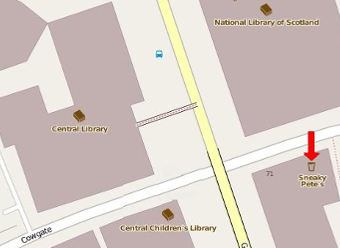
\includegraphics[width=8.5cm]{figures/with-zoom.jpg}\\[0pt]
\caption{Map with a more detailed zoom level}
\label{fig-with-zoom}
\end{center}
\end{figure}


%%%%%%%%%%%%%%%%%%%%%%%%%%%%%%%%%%%%%%%%%%%%%%%%%%%%%%%%%%%%%%%%%%%%%%%%%%%%%%%%%%%%%%%%%%%%%%%%%%%%%%%%%%%%%%%%%%%%%%%%%%%%%%%%%%%%%%%%%%%%%%%%%%%%%%%%%%
\section{Evaluation}
%%%%%%%%%%%%%%%%%%%%%%%%%%%%%%%%%%%%%%%%%%%%%%%%%%%%%%%%%%%%%%%%%%%%%%%%%%%%%%%%%%%%%%%%%%%%%%%%%%%%%%%%%%%%%%%%%%%%%%%%%%%%%%%%%%%%%%%%%%%%%%%%%%%%%%%%%%
\label{sec-eval}

In this section we illustrate the use of the Zoom corpus as training and test data for a machine learning approach to REG adapted from \cite{thiago-svm}. The  goal of this evaluation is to provide reference results for future comparison with purpose-built REG algorithms, and not to present a complete REG solution for this or other domains.

%................................
\subsection{Computational model}
%................................

The present model consists of 12 binary classifiers representing whether individual referential attributes should be selected for inclusion in an output description. The classifiers correspond to atomic attributes of the target and first landmark object ({\em type}, {\em name} and {\em others}), and relations. Referential attributes of other landmark objects were not modelled due to data sparsity and also to reduce computational costs. For similar reasons, the multivalue {\em between} relation is also presently disregarded, and `corner' relations involving two landmarks (e.g., two streets) will be modelled as two separate classification tasks.

Two learning features were considered by each classifier: {\em landmarkCount}, which represents the number of landmark objects near the main target, and {\em DistractorCount}, which represents the number of objects of the same type as the target within the relevant context in the map.

From the outcome of the 12 binary classifiers, a description is built by considering atomic target attributes in the first place. For every positive prediction, the corresponding atomic attribute is selected for inclusion in the output description. Next, relations are considered. If no relation is predicted, the algorithm terminates by returning an atomic description  of the main target object. If the description includes a relation, the related landmark object is selected  as well, and the algorithm is called recursively to describe the next object.

Since every attribute that corresponds to a positive prediction is always selected, the algorithm does not regard uniqueness as a stop condition. As a result, the output description may convey a certain amount of overspecification.


%......................
\subsection{Procedure}
%......................

We used a subset of singular descriptions from the Portuguese portion of the corpus. This comprises  821 descriptions produced in 9 scenes. Evaluation was carried out by comparing the corpus description with the system output to measure overall accuracy (i.e., the number of exact matches between the two descriptions), Dice \cite{dice} and MASI \cite{masi} coefficients (i.e., the degree of overlap between the algorithm output and the corresponding corpus description).

Following \cite{thiago-svm}, we built a REG model using support vector machines with radial basis function kernel. The classifiers were trained and tested using 6-fold cross validation. Optimal parameters were selected using grid search as follows: for each step in the main cross-fold validation, one fold is reserved for testing, and the remaining $k-1$ folders are subject  to a second cross-validation procedure in which different parameter combinations are attempted. The $C$ parameter is assigned the values 1, 10, 100 and 1000, and $\gamma$ is assigned 1, 0.1, 0.001 and 0.0001. The best-performing parameter set is selected to build a classifier trained from the $k-1$ folders, and tested on the test data. This procedure is repeated for every iteration of the main cross-validation procedure.


%......................
\subsection{REG Results}
%......................

Table \ref{tab-reg-results} summarizes the results obtained by the REG algorithm built from SVM classifiers, those obtained by a baseline system representing a relational extension of the Dale \& Reiter Incremental Algorithm, and by a Random selection strategy.  


% these results are for SVM.All.VAR-   compared to the AEI- baseline
\begin{table}[ht]
\begin{center}
\caption{REG results}
\label{tab-reg-results}
\begin{tabular} {  l c c c }
\hline
{Algorithm}							& {Acc.} 	& { Dice}		& MASI \\ \hline 
SVM											& 0.15		&	0.51			& 0.28 \\
Incremental							& 0.04		&	0.53			& 0.21 \\
Random selection       	& 0.03    & 0.45      & 0.15 \\
\hline
\end{tabular}
\end{center}
\end{table}

In what follows we compare accuracy scores obtained by every algorithm pair using the chi-square test, and we compare {\em Dice} scores using {\em Wilcoxon's} signed-rank test.

In terms of overall accuracy\footnote{And also in terms of MASI scores, although this is presently not further discussed.}, the SVM approach outperforms both alternatives. The difference from the second best-performing algorithm (i.e., the Incremental approach) is highly significant ($\chi^{2}=$ 79.87, df=1, p$<$0.0001). Only in terms of Dice scores an opposite effect is observed (T=137570.5, p$=$ 0.01413). 

We also assessed the performance of the individual classifiers. Table \ref{tab-svm-results} shows these results as measured by precision (P), recall (R), F1-measure (F1) and area under the ROC curve (AUC). 

%these are the rsults for the training over the set of ALL speakers 
\begin{table}[ht]
\begin{center}
\footnotesize{
\caption{Classifier results}
\begin{tabular}{l c c c c }
\hline
{{Classifier}}	& {P} & {R} & {$F_{1}$} & {AUC} \\
\hline
{{tg\_type}} 			& 0.95 & 1.00 & 0.98 & 0.25 \\
{{tg\_name}}			& 0.09 & 0.05 & 0.07 & 0.41 \\
{{tg\_other}}			& 0.00 & 0.00 & 0.00 & 0.05 \\                               
{{lm\_type}}			& 0.93 & 1.00 & 0.96 & 0.44 \\                               
{{lm\_name}}			& 0.97 & 1.00 & 0.98 & 0.35 \\                               
{{lm\_other}}			& 0.00 & 0.00 & 0.00 & 0.43 \\                               
{{next-to}}				& 0.50 & 0.24 & 0.32 & 0.63 \\                               
{{right-of}}			& 0.00 & 0.00 & 0.00 & 0.28 \\                               
{{left-of}}				& 0.00 & 0.00 & 0.00 & 0.27 \\                               
{{in-front-of}}		& 0.00 & 0.00 & 0.00 & 0.42 \\                               
{{behind-of}}			& 0.00 & 0.00 & 0.00 & 0.17 \\                               
{{in/on/at}} 			& 0.60 & 0.60 & 0.60 & 0.61 \\                               
\hline                   
\end{tabular}
\label{tab-svm-results}
}
\end{center}
\end{table}
\normalsize

From these results we notice that highly frequent attributes (e.g., type and name) were classified  with high accuracy, whereas others (e.g., multivalue attributes and relations) were not. 



%%%%%%%%%%%%%%%%%%%%%%%%%%%%%%%%%%%%%%%%%%%%%%%%%%%%%%%%%%%%%%%%%%%%%%%%%%%%%%%%%%%%%%%%%%%%%%%%%%%%%%%%%%%%%%%%%%%%%%%%%%%%%%%%%%%%%%%%%%%%%%%%%%%%%%%%%%	       >2
\section{Final remarks}
%%%%%%%%%%%%%%%%%%%%%%%%%%%%%%%%%%%%%%%%%%%%%%%%%%%%%%%%%%%%%%%%%%%%%%%%%%%%%%%%%%%%%%%%%%%%%%%%%%%%%%%%%%%%%%%%%%%%%%%%%%%%%%%%%%%%%%%%%%%%%%%%%%%%%%%%%%	       >2
\label{sec-final}

This paper has introduced the Zoom corpus of natural language descriptions of map locations. The corpus takes into account a domain that is significantly closer to real-world applications, and addresses more complex situations of reference than existing resources of this kind. In particular, the Zoom domain makes use of  contexts with different levels of detail, and contains instances of singular and plural reference produced by a relatively large number of speakers in both Spanish and Portuguese languages.

Preliminary results of a SVM-based approach to REG - which were solely presented for the future assessment of REG algorithms based on Zoom data - hint at the actual complexity of the REG task in this domain in a number of ways. 

First, we notice that a similar SVM-based approach in \cite{thiago-svm} on GRE3D3 and GRE3D7 data has obtained considerably higher mean accuracy (0.46 and 0.64 respectively) and higher mean Dice scores (0.78 and 0.89 respectively). This is of course explained by the increased complexity of the Zoom domain (e.g., in number of objects and possible atomic and relational properties etc.). However, we notice also that the Zoom annotation scheme - although taking into account an already large number of possible attributes - is still overly simple. In particular, the attribute {\em others} has been overused and, as a result, the chances of reproducing the corpus descriptions is narrow. Clearly, more work needs to be done to expand the annotation scheme and split {\em others} into a larger number of attributes.

Second, Zoom descriptions are prone to convey relations between a single target and multiple landmark objects, as in `the restaurant on 5th street, near the library'. Although common in language use, the use of multiple relational properties in this way has been little investigated, perhaps because it may lead to ambiguous descriptions, as in `the restaurant near the church on Jackson street and the bar on 5th street' for a restaurant located near the junction of these two streets.

As future work, we intend to make the corpus publicly available for research on multiple aspects of content selection and surface realisation in REG. In particular, we envisage the use of the Zoom corpus as training and test data for machine learning models of REG, and also to address further issues that have not been addressed in the present paper. These include  the generation of referring expressions from knowledge bases with different degrees of detail, and the issues of between-speakers and within-speakers variation in REG.


%..........................
\section*{Acknowledgements}
%..........................
This work has been supported by anonymous. 

\clearpage
\bibliographystyle{named}
\bibliography{mainZoom}   % name your BibTeX data base

\end{document}
